We saw in previous lectures that the MEL heater experiment
\begin{center}
\begin{tikzpicture}
\draw[pattern=bricks]  (-3,-2) -- ++(0,.25) -- ++(10,0)  -- ++(0,-.25) --  cycle;
\draw[pattern=bricks]  (-3,-1) -- ++(0,.25) -- ++(1,0) -- ++(0,1.75) -- ++(8,0) -- ++(0,-1.75) -- ++(1,0) -- ++(0,-.25) -- ++(-1.25,0) -- ++(0,1.75) -- ++(-7.5,0) -- ++(0,-1.75) -- ++(-1,0) -- cycle;

\draw (2,-1.45) node {Chamber heat capacity: $C$, air specific heat: $c$};
\draw (2,-2.25) node {Thermal Resistance: $R$};
\draw (2,-3.25) node {Ambient Temperature: \tikz[baseline=-2pt] \node[circle,fill=yellow,inner sep=1pt] {$T_{a}$};};
\draw (2,0) node[circle,fill=pink,inner sep=1pt] {$T_{o}$};
%\draw (4,0.25) node[circle,draw=gray,line width=2pt,inner sep=1pt,outer sep=0pt] (th1) {$T_{1}$};
\draw (5,0.25) node[circle,fill=green,draw=gray,line width=3pt,inner sep=1pt,outer sep=0pt] (th2) {$T_{1}$};

%\draw[very thick] (th1) -- ++(0,1.5);
\draw[very thick] (th2) -- ++(0,1.5);

\draw[->] (-4,-1.5) node {$\begin{matrix}\dot{m}\\\mbox{\tikz \node[circle,fill=yellow,inner sep=1pt] {$T_{a}$};}\end{matrix} $} -- ++(1,0); 

\draw (0,0) node[inner sep=0,outer sep=0] (coil) {\input{\mainfolder/DrawingElements/CircuitElements/inductor.tex}};
\draw[very thick] (coil.0) -- ++(.01,0) -- ++(0,2);
\draw[very thick] (coil.180) -- ++(-.01,0) -- ++(0,2);
\draw[->,thick=15pt] (0,.25) -- ++(0,-1) node[right=2pt] {$\dot{Q}_{i}$};

\end{tikzpicture}\end{center}
has thermal circuit
\begin{center}
\begin{tikzpicture}
\draw (0,0) node[draw,fill,inner sep=0pt,outer sep=0pt,circle] (Ta) {$\rule{2pt}{0pt}$};
\draw (Ta.0) node[above left=4pt,circle, inner sep=1pt,fill=yellow] {$T_{a}$};
\draw (3,0) node[draw,fill,inner sep=0pt,outer sep=0pt,circle] (To) {$\rule{2pt}{0pt}$};
\draw (To.0) node[above right=4pt,circle, inner sep=1pt,fill=pink] {$T_{o}$};
\draw (7,0) node[draw,fill,inner sep=0pt,outer sep=0pt,circle] (T1) {$\rule{2pt}{0pt}$};
\draw (T1.0) node[above=4pt,circle, inner sep=1pt,fill=green] {$T_{2}$};
\draw (3,-3) node[draw,fill,inner sep=0pt,outer sep=0pt,circle] (Tref) {$\rule{2pt}{0pt}$};
\draw (Tref.0) node[below=2pt,circle,inner sep=1pt] {$T_{ref}$};

\draw (1.5,0) node[inner sep=0,outer sep=0] (R1) {\input{\mainfolder/DrawingElements/CircuitElements/resistor.tex}};
\draw (0,-1.5) node[inner sep=0,outer sep=0] (V1) {\input{\mainfolder/DrawingElements/CircuitElements/voltagesource.tex}};
\draw (1.5,1) node[inner sep=0,outer sep=0] (R2) {\input{\mainfolder/DrawingElements/CircuitElements/resistor.tex}};
\draw (3,-1.5) node[inner sep=0,outer sep=0,rotate=90] (C1) {\input{\mainfolder/DrawingElements/CircuitElements/capacitor.tex}};
\draw (4,-1.5) node[inner sep=0,outer sep=0] (I1) {\input{\mainfolder/DrawingElements/CircuitElements/currentsource.tex}};
\draw (5.5,0) node[inner sep=0,outer sep=0] (Rt) {\input{\mainfolder/DrawingElements/CircuitElements/resistor.tex}};
\draw (7,-1.5) node[inner sep=0,outer sep=0,rotate=90] (C2) {\input{\mainfolder/DrawingElements/CircuitElements/capacitor.tex}};

\draw (C1) node[left=12pt] {$C$};
\draw (C2) node[right=12pt] {$C_{T}$};
\draw (Rt) node[above=8pt] {$R_{T}$};
\draw (R1) node[above=8pt] {$R$};
\draw (R2) node[above=8pt] {$R_{v}$};
\draw (V1) node[left=12pt] {$T_{a}$};
\draw (I1) node[right=12pt] {$\dot{Q}_{i}$};

\draw[very thick] (V1) -- (Ta);
\draw[very thick] (Ta) |- (R2.180);
\draw[very thick] (Ta) -- (R1.180);
\draw[very thick] (To) |- (R2.0);
\draw[very thick] (To) -- (R1.0);
\draw[very thick] (To) -- (C1.0);
\draw[very thick] (To) -- (Rt.180);
\draw[very thick] (T1) -- (Rt.0);
\draw[very thick] (T1) -- (C2.0);
\draw[very thick] (C2.180) |- (Tref);
\draw[very thick] (V1.-90) |- (Tref);
\draw[very thick] (Tref) -- (C1.180);
\draw[very thick] (I1.90) -- (To);
\draw[very thick] (I1.-90) -- (Tref);

\end{tikzpicture}
\end{center}
You are going to design a PD controller  for this system. You will measure the temperature reading of the thermocouple, compare it to a reference, and then use the PD controller to calculate the required voltage to a voltage controlled heater. The voltage input is $v_{h}$ and the heat flux is given by $\dot{Q}_{i}=K_{h}v_{h}$. The block diagram of your control system is as follows:
\begin{center}
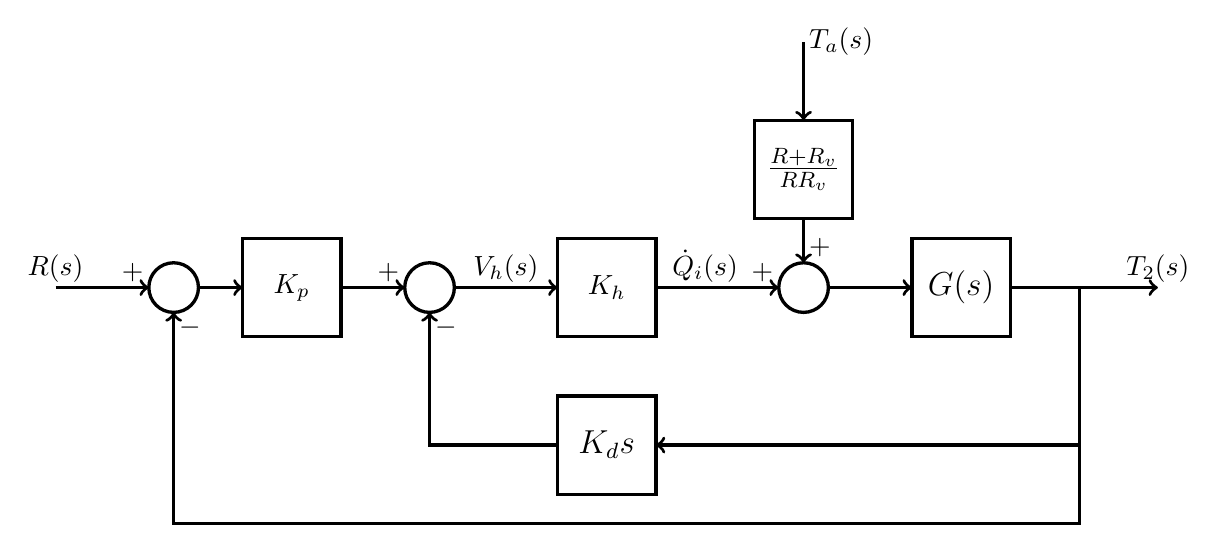
\begin{tikzpicture}[scale=1,inner sep=0pt,outer sep=0pt,very thick,
sysblock/.style={draw,rectangle,inner sep=2pt,minimum width=1.25cm,minimum height=1.25cm,very thick}]
\draw (-2,0) node[draw,circle] (sum1) {$\rule{0pt}{18pt}$};
\draw (-.5,0) node[sysblock] (Kp) {$\large K_{p}$};
\draw (1.25,0) node[draw,circle] (sum3) {$\rule{0pt}{18pt}$};
\draw (3.5,0) node[sysblock] (Kp2) {$\large K_{h}$};
\draw (6,0) node[draw,circle] (sum2) {$\rule{0pt}{18pt}$};
\draw (8,0) node[sysblock] (G) {\large $G(s)$};
\draw (3.5,-2) node[sysblock] (Kd) {\large $K_{d}s$};
\draw (6,1.5) node[sysblock] (F) {\large $\frac{R+R_{v}}{RR_{v}}$};
\draw[->] (-3.5,0) node[above=2pt] {$R(s)$} -- (sum1.180) node[above left=2pt] {$+$};
\draw[->] (sum1.0) --   (Kp);
\draw[->] (Kp) -- (sum3.180) node[above left=2pt] {$+$};
\draw[->] (sum3.0) -- node[pos=.5,above=2pt] {$V_{h}(s)$} (Kp2);
\draw[->] (Kp2) -- node[pos=.4,above=2pt] {$\dot{Q}_{i}(s)$}   (sum2.180) node[above left=2pt] {$+$};
\draw[<-] (sum2.90) node[above right=2pt] {$+$} -- (F.-90);
\draw[<-] (F.90) -- ++(0,1) node[right=2pt] {$T_{a}(s)$};
\draw[->] (sum2) -- (G);
\draw[->] (G) -- ++(2.5,0) node[above=2pt] {$T_{2}(s)$};
\draw[->] (G) ++(1.5,0) -- ++(0,-3) -| (sum1.-90) node[below right=2pt] {$-$};
\draw[->] (G) ++(1.5,0) ++(0,-2) -- (Kd.0);
\draw[->] (Kd.180) -| (sum3.-90) node[below right=2pt] {$-$};

\end{tikzpicture}
\end{center}

where $G(s)=\frac{T_{2}(s)}{\dot{Q}_{i}(s)}$. The system parameters are $R_{v}=R=2$, $C=1$, $R_{T}=0.1$, $C_{T}=0.1$, $K_{h}=1$. 
\begin{enumerate}
\item Find $G(s)$.
\item Design a PD control so that a unit step command from $R(s)$ has rise time $t_{r}=0.1$s and overshoot $\%OS=10\%$. For this design you can assume $T_{a}(s)=0$. 
\item Confirm your design by finding the closed loop transfer function from $R(s)$ to $T_2(s)$ and using \textsc{Matlab} to plot the step response (See Lecture 12, section 4). 
\item Find the steady state error for a one degree change in the ambient temperature $T_{a}$.
\end{enumerate}
